\documentclass[conference]{IEEEtran}
\IEEEoverridecommandlockouts
% The preceding line is only needed to identify funding in the first footnote.
% If that is unneeded, please comment it out.
\usepackage{amsmath,amssymb,amsfonts}
\usepackage{algorithmic}
\usepackage{graphicx}
\usepackage{textcomp}
\usepackage{xcolor}
\usepackage[numbers]{natbib}
\usepackage{graphicx}

\usepackage{todonotes}
\newcommand{\cit}[1][]{\todo[tickmarkheight=0.2cm]{cit #1}}

\begin{document}

\title{Explainable AI and cognitive bias: why should we be careful in trusting AI explanations}

% \title{Trusting explanations: what can we expect from XAI?}

\author{\IEEEauthorblockN{Alvise de' Faveri Tron}
    \IEEEauthorblockA{\textit{Politecnico di Milano} \\
        alvise.defaveri@mail.polimi.it}}

\maketitle

\begin{abstract}
    Artificial Intelligence is known to suffer from explainability problems:
    it is often hard for humans to explain why an AI-based system took a
    particular decision or to understand what is the general logic behind its
    behavior.
    This issue poses a serious ethical and technical barrier to the progress
    of AI, since the opacity of these algorithms has led, in some cases, to  systems that behave in a weird, unfair or dangerous way.
    XAI (short for eXplainable AI) is a research field
    that aims at solving this problem by providing some kind of explanation
    interface to humans that have to interact with AI systems.
    Although this has proven to be a good idea for some purposes and has generated useful tools, such as layer-per-layer visualization of the patterns that are being recognized in deep convolutional networks, there is also a potential risk associated to the creation of a complex intermediate explanation layer, since it is difficult to measure how our decisions are impacted by it. Human
    decision-making is in fact known to be affected by many cognitive bias, for instance the so-called \textit{framing effect}, which happens when our
    decisions are influenced by the way information is presented.
    If explanation interfaces are not carefully crafted they could, in principle, leverage this kind of cognitive bias to convince a human operator that the internal model is correct, or find a way of presenting it so that the predictions made by the AI are not questioned.
    % Considering that many XAI solutions focus on reducing the
    % \textit{complexity} of explanations, giving less importance to aspects
    % such as \textit{fidelity} or user understanding, which are much more difficult to measure, there is a real possibility of creating simple interfaces that sound convincing but are not completely accurate. If not counterbalanced by an comprehensive evaluation process, which is lacking today in XAI, could this create an incentive for creating explanation interfaces that are good at lying?
    % Such
    % behaviors are extremely problematic if we think about which fields are
    % starting to adopt AI as a support for human decisions - in particular the
    % legal and medical field.
    % Although many solutions have been proposed in this research framework, there is still a lack of a formal definition of \textit{interpretability}, which means that each researcher gets to choose its own metric over which the explanation quality is evaluated.
    % Many studies for example focus on the explanation \textit{complexity}, while on the other hand many argue this is not enough to define how good is an explanation. In particular, I want to focus on the fact that ignoring how faithfully an explanation represents the original model and how good it communicates it to the end user might lead to the creation of explanation interfaces that can leverage known human cognitive biases, such as the framing effect, to convince humans. In this case, there is a very thin line between being able to present information in a convincing way and lying.
\end{abstract}

% 1. why is black box a problem for AI
% ethical
% technical
% 2. AI suffers from interpretability problems
% both users and developers of this technology generally don't fully understand how it works.

% 3. XAI
% goals
% proposed solutions
% 4. no common definition of interpretability
% both because of the subjective nature of explanations
% and because of the different possible users and goals that an explanation can have
% 5. metrics


% 6. is there a tradeoff between complexity and fidelity
% yes
% Framing effect
% possible consequences
% critiques

%-----------------------------------------------------------------%
\section{Introduction}
\label{sec:intro}

\todo[inline]{add comment on interpretability vs explainability}
\todo[inline]{add comment on the fact that internals are useful only to developers}

AI has made giant steps since its birth in the late 1950s, especially in the last
decade. Many tasks that in the past were exclusively carried out by humans, for
example in the legal, law enforcement and medical fields, are now being
automated with AI.  \cit This increase in AI's capabilities is a game-changer for
technology and society, so much that expressions like ``AI singularity'' \cit
have been used to describe this
phenomenon.

However, today's AI is far from being perfect: many decision systems based on AI
still fail at tasks that are considered easy for humans, such as identifying
objects in images or extracting salient information from text, and our
understanding of this technology is still partial and prone to
errors.

One well known issue of modern AI-based decision systems is that they are
difficult to debug, partly because many aspects of their behavior are not in
direct control of the developer. Even when a decision system behaves well in a
set of test cases, it is difficult to understand if the internal model correctly
reflects the intended one. Machine Learning applications in particular tend to
suffer from biases \cit that are difficult to spot during the test phase, and they
tend to display an overall opaque behavior which is not easily understandable
for humans: this is known as the \textit{black box problem} in AI \cit, and it
poses huge ethical and practical concerns about whether we can trust this
technology or not, especially given the nature of the tasks we expect it to be
able to undertake in the future.

Explainable Artificial Intelligence (XAI) is a field of AI that aims at
addressing the problem of understanding AI and making it more reliable and
trustworthy. Many interesting results have been achieved in this field, and many
more are expected to come in the next years. However, there are still some
fundamental aspects that this approach seems to struggle with.

One of them is
the problem of giving a formal and comprehensive definition of interpretability, which is a quite
discussed topic in the field. \cit This lack of a common definition has led
many researchers to concentrate only on partial aspects such as the
explanation's \textit{complexity}, which is a relatively easy aspect to measure
when using proxies such as the number of elements that compose the explanation.

More difficult yet essential aspects to evaluate should be the explanation's
\textit{fidelity}, i.e. the adherence of the explanation to the original system, and its \textit{informativeness}, which is the ability to transfer to the user a faithful representation of the internal model.
But since fidelity and complexity are often in contrast when devising explanation systems, it is easy to image that the generation of a simple explanation for a complex decision can lead to omitting some aspects, that may or may not be important for evaluating it.

Taking this approach to its extreme consequences, I want to argue that a system where fidelity is never taken into account and the only metric is user feedback on the clarity of the explanation can lead to a preference for
those systems that can cover their defects better than others with respect to
the specific explanation interface in use. This can be especially harmful for ``thick'' explanation layers that try to bridge the gap between human thinking and machine learning systems, which are generally very different. If these explanation systems are able to leverage human cognitive biases, which are known to exist in this kind of situations, to sound more convincing, we could end with machines that are actually incentivezed to lie.

The final goal of this paper is to offer a reflection on how complex the
evaluation process for XAI systems is, and how dangerous are the consequences of underestimating the biases that an explanation can introduce in the decision process in which they are involved.

% In particular, there seems to be a lack of uniform terminology across the
% research community when it comes to XAI. There have been attempts to define the
% notions of ``interpretability'', ``explainability'' along with
% ``reliability'',``trustworthiness'' and other similar notions, but there is no
% general consensus on how to formally define and measure these properties.
% \cit

% In this paper we want to highlight how the lack of a formal definition of
% ``explainability" for XAI is not just due to a lack of standardization in this
% newborn field, but some aspects of this problem have their roots in profound
% questions about intelligence, thought and cognition, which are still mainly
% unsolved today. We will try to propose a conceptual framework to define
% ``explainability'', identifying some of the problem's dimensions, in order to
% analyze those aspects that are not related to a specific solution. We will
% highlight how the problem of measuring these dimensions is more than just a
% technical problem, and that the subjective nature of explainability can cause
% cognitive biases to be accentuated in the interpretation of an AI output.

% In this context, we will use  the words “explainability” and “interpretability”
% interchangeably, as suggested in \cit.

The reminder of this paper is organized as follows.

Section~\ref{sec:background} provides some background on the kind of problems that XAI tries to solve and a classification of the solutions that are currently being developed.

Section~\ref{sec:explainability} introduces the problem of defining
interpretability, and proposes a classification of the aspects that define an
explanation.

Section~\ref{sec:troubles} discusses the idea that explanation interfaces might be able to fool a human user into believing that a specific algorithm is doing the right thing.

Finally, Section~\ref{sec:conclusions} contains a list of possible critiques to
the ideas expressed in this paper and proposes possible improvements.

%-----------------------------------------------------------------%
\section{Background}
\label{sec:background}

\subsection{The need for interpretability in AI}
\label{sec:opaque}

Modern complex AI techniques, such as deep learning and genetic algorithms, are naturally opaque \cit [24], yet they constitute the foundations of today's image and speech recognition, natural language processing, autonomous driving and many other intelligent systems. These are the kind of algorithms which are being considered in this paper.

As this technology advances, we are starting to see the problems that derive from its opacity. In the 2010s public concerns about racial and other bias in the use of AI for criminal sentencing decisions and findings of creditworthiness have led to increased demand for transparent artificial intelligence. \cit [1] As a result, many academics and organizations are developing tools to help detect bias in their systems. \cit [22]

Marvin Minsky et al. raised the issue that AI can function as a form of surveillance, with the biases inherent in surveillance, suggesting HI (Humanistic Intelligence) as a way to create a more fair and balanced ``human-in-the-loop'' AI. \cit[23]

From a practical point of view, modern AI has been found to be particularly vulnerable to ``Clever Hans'' situations, in which an AI chooses the right answer for the wrong reason. A notorious example is \citet{cleverhans}, where the Fisher vector classifier trained on the PASCAL VOC 2007 data had learned to recognize horses by recognizing a copyright tag that was present in about one-fifth of the horse figures in the training dataset.

It is important to notice that the problems highlighted in the above examples
cannot be associated to any programming error of these systems, but is more of an inherent issues of these machines.

%-----------------------------------------------------------------%
% goals (introspection, human-in-the-loop, right for an explanation)
% scope (local vs global)
% techniques

\subsection{The XAI approach}
\label{sec:xai}

The term \textit{Explainable AI} refers to methods and techniques in the application of artificial intelligence that aim at improving the possibility for humans to understand its solutions. We can consider \citet{DARPA} as a starting point for modern XAI research. Figure~\ref{fig:xai} reports the goals of XAI as stated in that paper, which can be summarized as:

\begin{itemize}
    \item \textit{Accountability}: the possibility to identify precise responsibilities when things go wrong in AI.
    \item \textit{Transparency}: the possibility to understand the reasons why AIs behave in a certain way, for both debugging and trust purposes.
    \item \textit{Fairness}: the possibility to measure possible bias that has been picked up by the AI model.
\end{itemize}

\begin{figure}[h!] 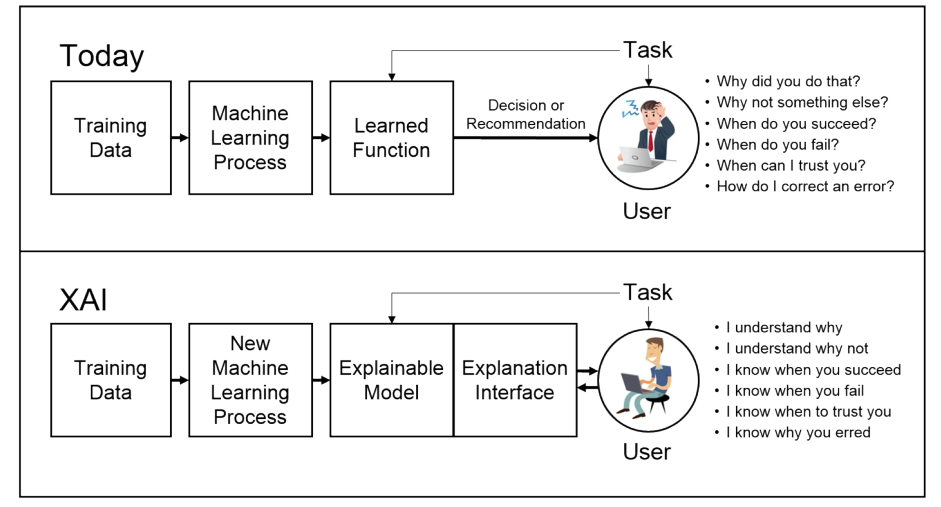
\includegraphics[width=\linewidth]{images/xai.png}
    \caption{The goals of XAI as expressed in \citet{DARPA}. } \label{fig:xai} \end{figure}


The creation of such systems requires the join effort of a variety of research
fields, from Computer Science to Cognitive Psychology, and there is still a lot
of work to do. Nevertheless already many papers have been submitted on the
subject, indicating a growing interest of the research community.

\subsection{Proposed Solutions}
\label{sec:solutions}

Given the variety of goals of in this field, many different solutions
have been proposed by various papers in the framework of XAI, which vary greatly
in intended use and adopted approach.
% \citet{Giannotti} proposes the following high-level classification for XAI techniques, as shown in Figure~\ref{fig:xaiclass}:

% \begin{itemize}
%     \item \textit{Model explanation}: Global explanation of the whole model's behavior.
%     \item \textit{Outcome explanation}: Local explanation of a single outcome.
%     \item \textit{Model inspection}: Explanation trough introspection of the model's internals.
%     \item \textit{Transparent Box design}: Making AI easier to understand by design, e.g. by using algorithms that are intrinsically clearer for humans.
% \end{itemize}

% \begin{figure}[h!] 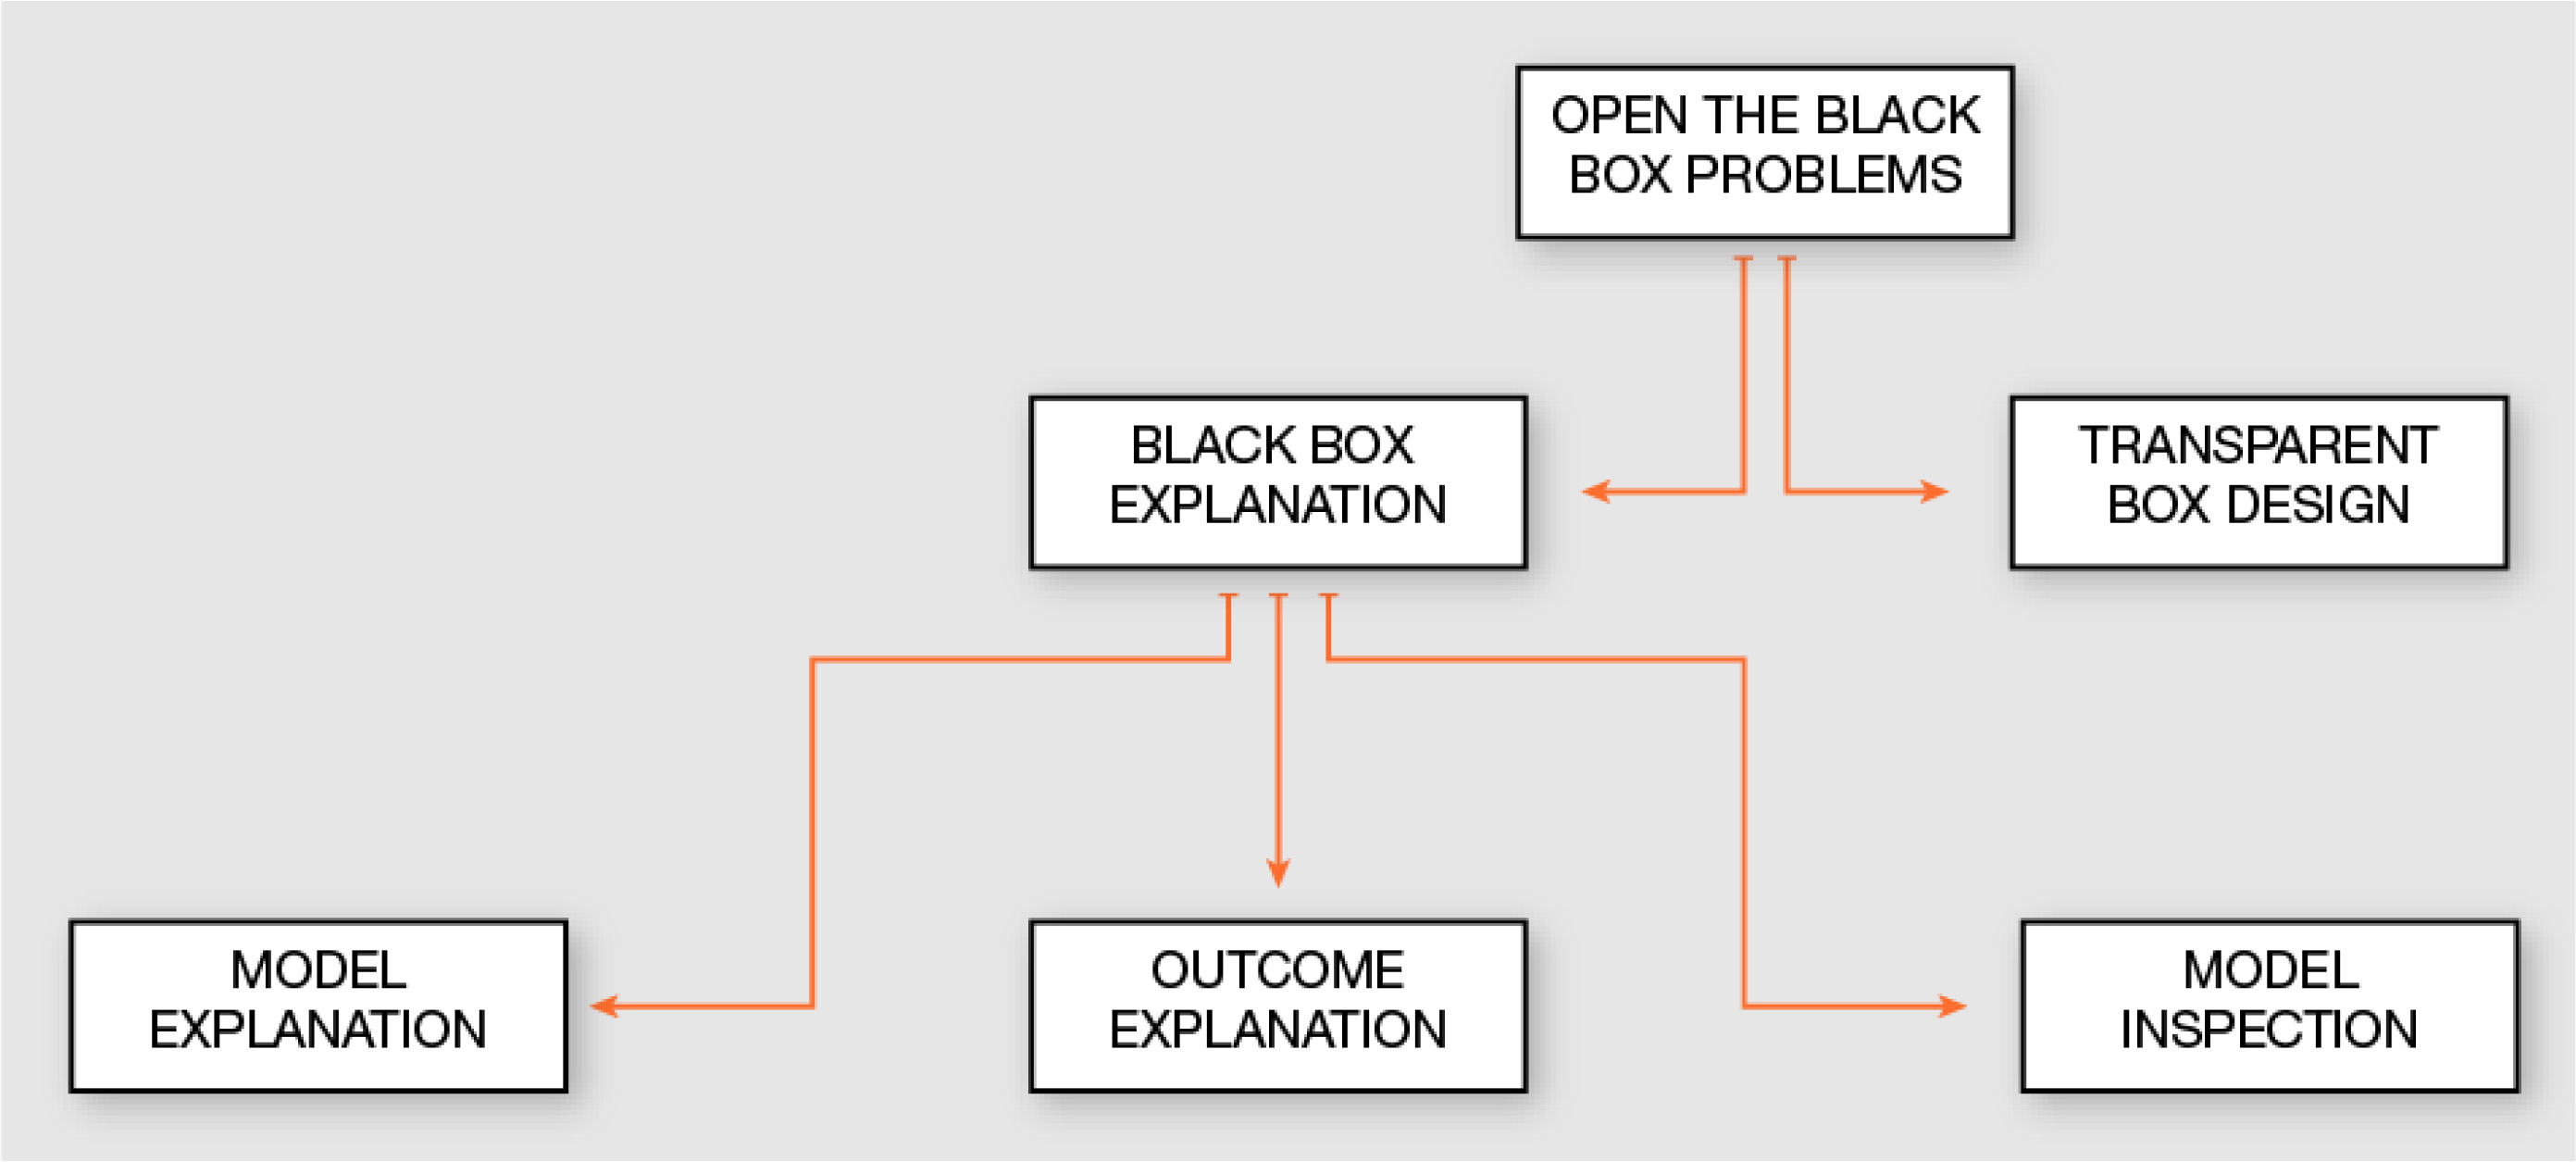
\includegraphics[width=\linewidth]{images/xaiclass.png}
%     \caption{Taxonomy of XAI solutions provided by \citet{Giannotti}} \label{fig:xaiclass} \end{figure}

This paper focuses is in particular on those methods that are based on
reverse-engineering already existing models, also called \textit{post-hoc
    interpretability}, to create an explanation. This kind of systems are the ones
that are being mostly developed in the current XAI framework
(\citet{Giannotti}).

Existing solutions of this type might be classified referring to \citet{nasaxai}:

\begin{enumerate}
    \item \textit{Visualization}: these approaches focus on finding an effective
          way to visually represent key aspects of the AI
          behavior. One example is to use \textit{saliency masks}, such as the
          one in Figure~\ref{fig:heatmap}, to highlight which are the most
          significant portions of the input for the AI model.

          \begin{figure}[h!] \centering 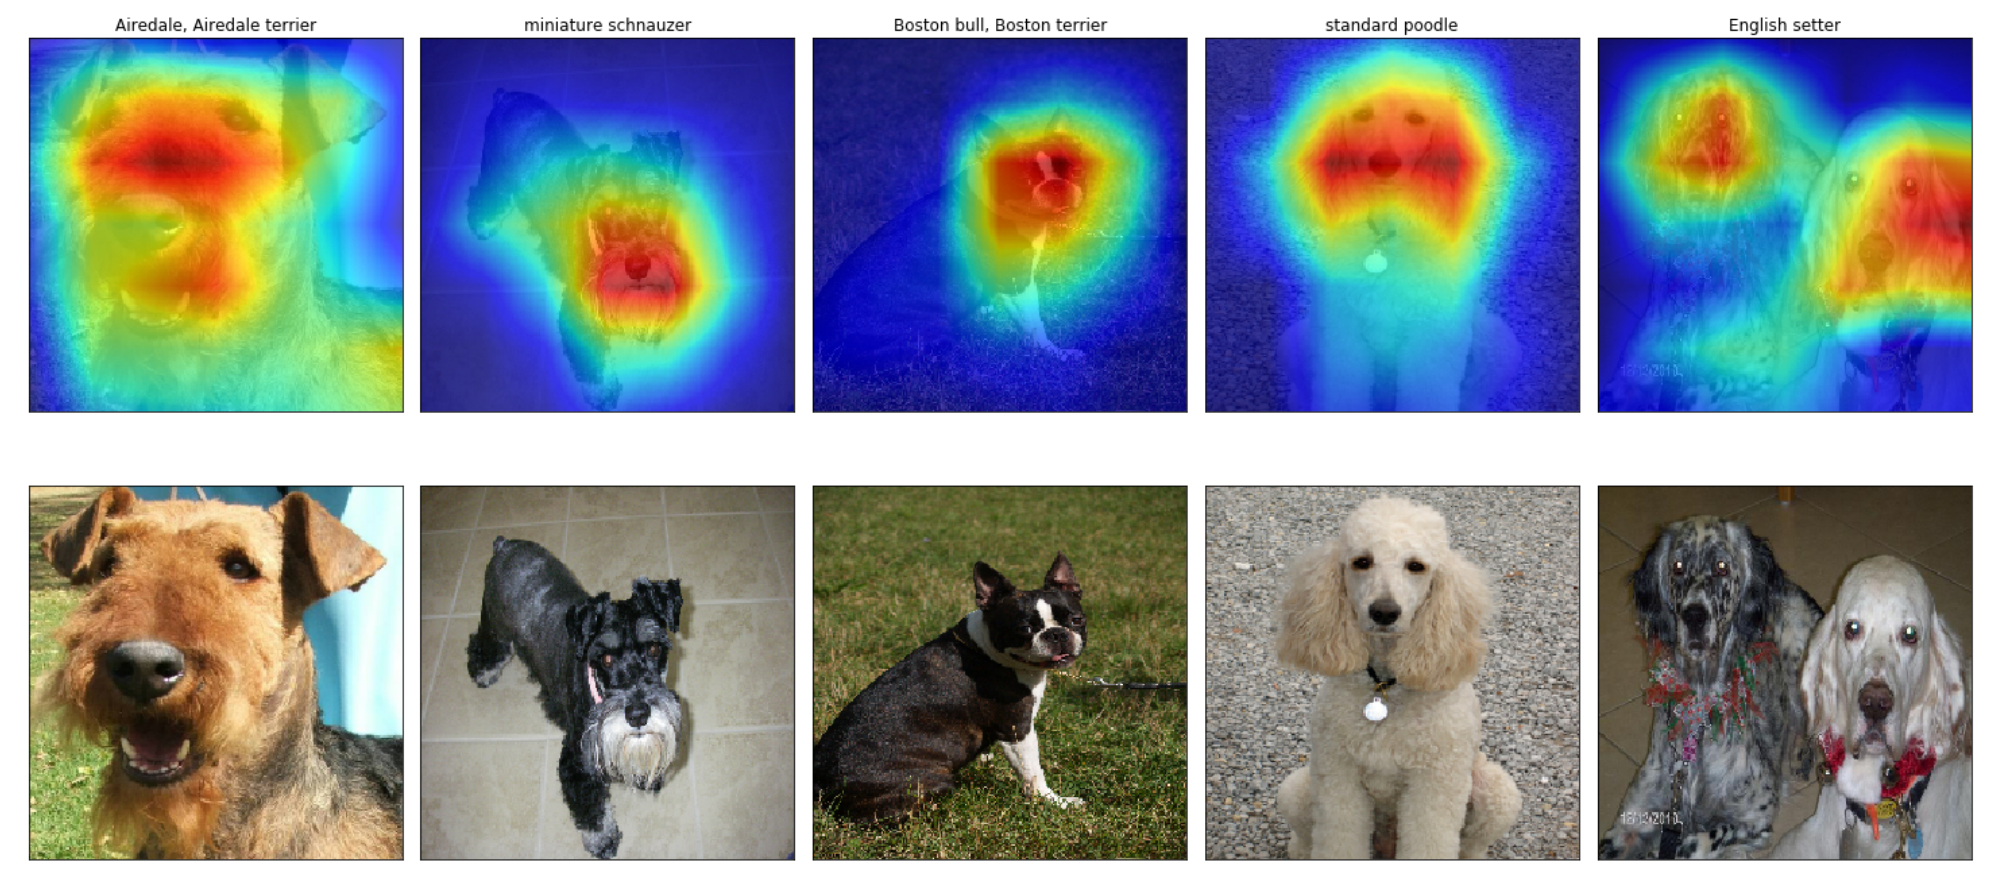
\includegraphics[width=0.9\linewidth]{images/dog_localization.png}
              \caption{An example of a heatmap representing the importance of pixels for a given classification decision, from blue (low importance) to red (high importance). } \label{fig:heatmap} \end{figure}

    \item \textit{Approximation}: this approach consists in using simple models for the explanation, or simplifying already existing models to just a set of important features. This is the case of \textit{single tree approximation} \cit, where the internal structure of an AI algorithm is approximated to a singe classification tree, such as in Figure~\ref{fig:dectree}.

          \begin{figure}[ht!] \centering
              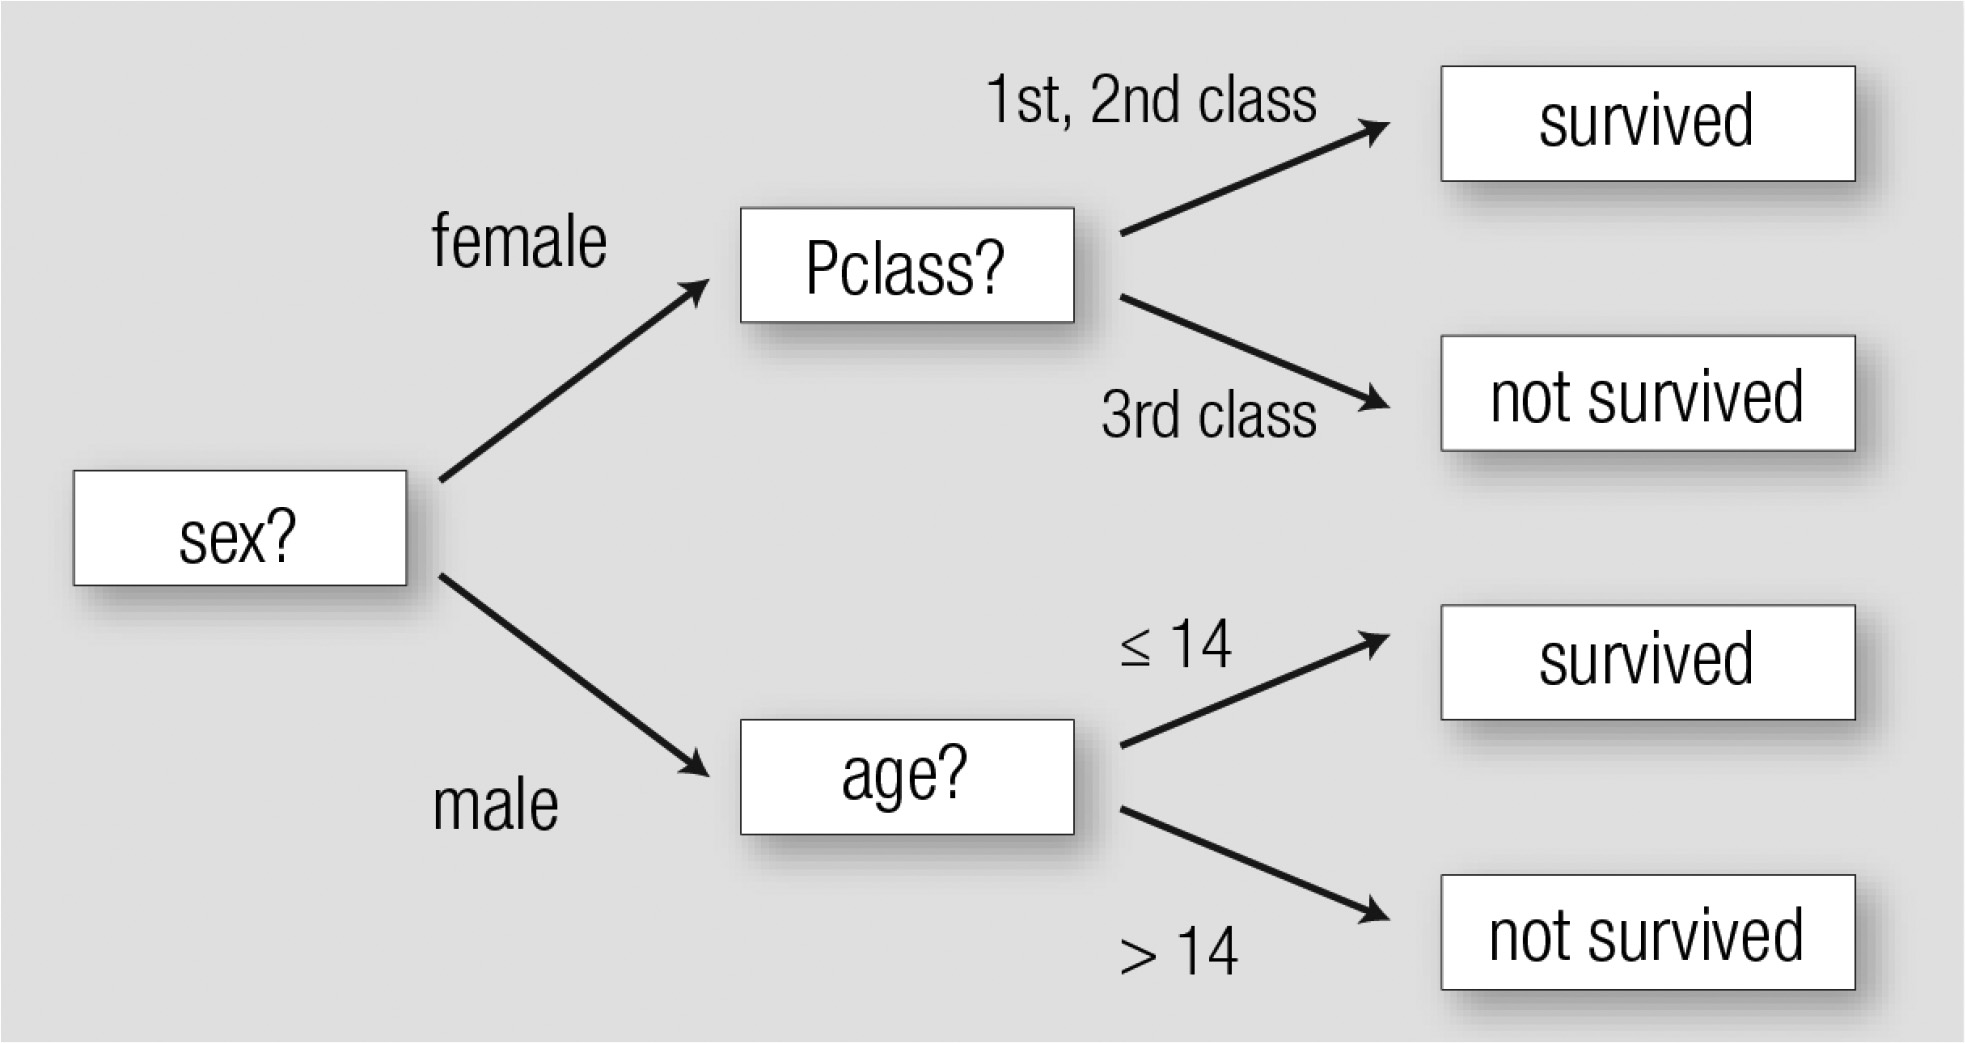
\includegraphics[width=0.9\linewidth]{images/dectree} \caption{A simple Decision Tree} \label{fig:dectree} \end{figure}

    \item \textit{Causal Models (CAMEL)}: \cit the idea of this approach is to generate causal explanations of ML operation and present them to the user as intuitive narratives in an interactive, easy-to-use interface grounded in cognitive engineering theories. A scheme of the architecture needed for this approach is illustrated in Figure~\ref{fig:camel}.

          \begin{figure}[ht!] \centering
              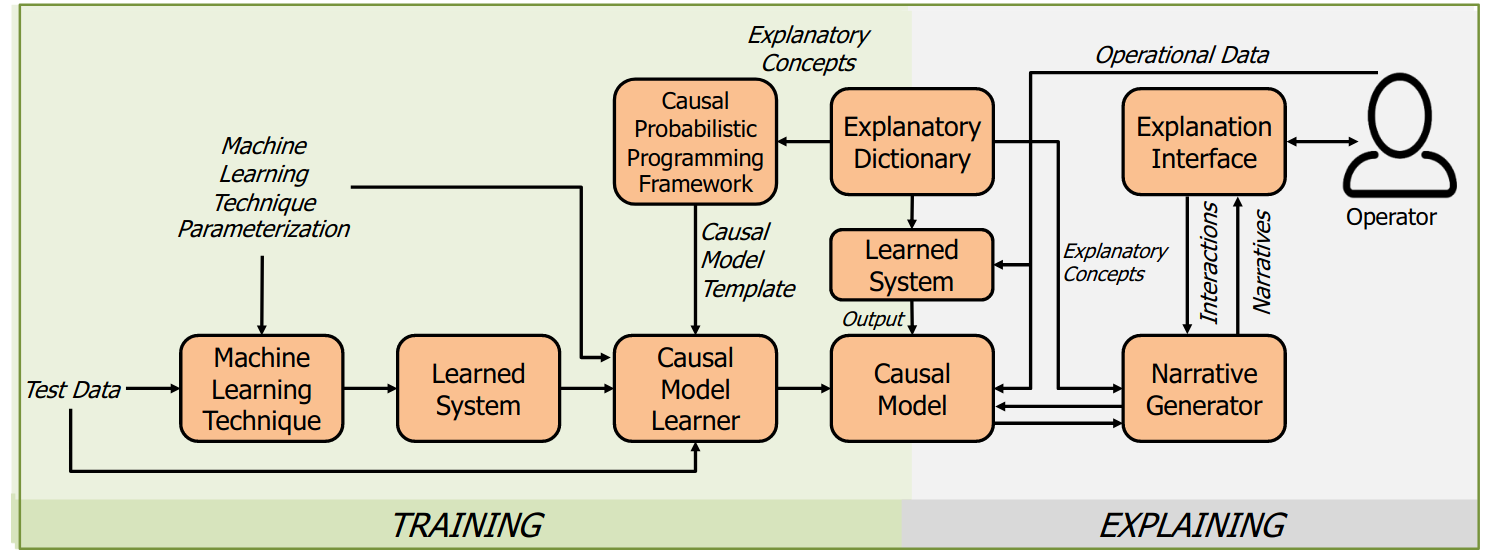
\includegraphics[width=0.9\linewidth]{images/camel.png} \caption{Architecture of the CAMEL approach.} \label{fig:camel} \end{figure}

    \item \textit{Learning and Communicating Explainable Representations}: explanations themselves are learned as a separate part of the training process.

    \item \textit{Explanation by Example}: a nice information to have when
          trying to understand an AI model, especially in the case of
          classifiers, is an example, or a \textit{prototype}, of how the AI
          thinks that a typical member of a given class should appear and/or which characteristics should be changed to change the outcome of the classifier.
\end{enumerate}

While solutions of type 1 (Visualization) give a clear insight on what the AI model is actually doing, they are really effective only in image-based applications. Other types of explanations are more general, but more problematic. In particular, solutions of type 2 (Approximation) suffer from the possibility of over-simplification, which could be misleading, and don't directly represent the internals of the AI model. Solutions of type 3 (Causal Models) are even more distant from the original model, as they try to bridge human-like causal reasoning and statistical correlation, which is the way in which machine learning algorithms generally work. Solutions of type 4 (Learning) add another dimension to this problem, since there is the possibility for machines to \textit{learn} the explanation representation.

These examples already show how the problem of interpretability has multiple dimensions, and the closer we try to get to human reasoning and focus on the user's thinking process, the less we are being explicit on the AI's internals and what is really happening inside the black-box.

%-----------------------------------------------------------------%
\section{Defining Explainability}
\label{sec:explainability}

As anticipated in Section~\ref{sec:intro}, one fundamental problem in
the field of XAI is that there is no single conventional notion of
explainability.
\citet{mythos} goes as far as considering the term itself ill-defined, therefore
stating that claims about interpretability generally have a quasi-scientific
nature. \citet{Giannotti} on the other hand, considers the lack of a mathematical description as an obstacle for the
future development of this field. \citet{DARPA} itself defines the
formalization of an evaluation metric for explanations as one of the goals of
the XAI project, to be developed in parallel with technical solutions.

When analyzing the problem of defining and evaluating interpretability, two questions naturally arise:

\

\textbf{Explainable to whom?} The concept of \textit{user} of an AI system is
not always well defined, nor is the concept of user of an explanation. This
might include:

\begin{itemize}
    \item The \textit{developer} of the AI system, as he is only partially in
          control of what the algorithm does
    \item The \textit{operator} of an AI system: many AI algorithms nowadays are
          being used as an input for a human to make decisions on a certain
          subject
    \item The \textit{end user} which is affected by the decision of an AI
\end{itemize}

\

\textbf{Explainable for which purpose?} Different users have different needs,
that can partially overlap, when it comes to AI explanation. More in general,
whether a certain representation can be considered explanatory depends to some
degree on what it is being used for. In the case of XAI, some common purposes
are:

\begin{itemize}
    \item \textit{Debugging}: finding errors and backtracking them to a specific reason
    \item \textit{Human-in-the-loop}: creating systems where human and AI
          decisions can co-exist and influence each other
    \item \textit{Validation}: understanding if a certain model is good enough
          to be deployed for a certain task, where it fails and what happens
          when it fails
    \item \textit{Appeal AI decisions}: \footnote{This goal is not
              explicitly listed in the original scope of XAI, but has
              gained traction recently with the introduction of the concept of \textit{right for an explanation} in Europe's new GDPR. (\citet{righttoexpl})} giving the right to
          users and citizens that are affected by AI decisions to know,
          understand and possibly appeal decisions that are automated with
          AI systems
\end{itemize}

\

It appears quite evident that different XAI solutions with different scopes and
intended users cannot be compared in the same way.

% If, on one hand, many solutions have already been proposed to tackle the
% problem, with various claims regarding their interpretability, on the other hand
% the lack of a formal definition seriously challenges the findings of these
% researches, casting a shade of doubt on the proposed solutions.

\subsection{Possible Metrics}
\label{sec:dimensions}

Bearing in mind the different goals that an XAI system can have, we can identify
a series of characteristics that are different among different solutions:

\begin{itemize}
    \item \textit{Complexity}: how many elements are there in the explanation?
    \item \textit{Clearness}: how cognitively hard is the explanation? How
          difficult is it to understand the correspondence between the elements
          of the explanation and the information we are trying to gain?
    \item \textit{Informativeness}: how much information, weighted on how
          meaningful is is, can be extracted by the explanation? E.g. does the
          explanation significantly modify the level of uncertainty about the AI
          behavior?
    \item \textit{Fidelity}: how closely does the explanation represent the
          internal functioning of the system? Are all the facts inferred from
          the explanation also applicable to the original system?
\end{itemize}

Clearly, each metric can be more or less important for specific use-cases, but there is also a difference in the way we can measure these characteristics.

Complexity, for instance, is often measured using a proxy such as the number of elements in the explanation, which can be for example the depth of the decision tree in those explanation interfaces that make use them. On the other hand, clearness and informativeness are more difficult to quantify a-priori, but could be empirically evaluated by providing explanations to a human control-group and verify how they respond.

In general, we can identify two ways of evaluating an AI explanation: one is using a direct measurement of some quantity that we can derive directly from the explanation. The second one is considering an explanation itself a black-box, and check if it actually provides a better understanding of the AI model to some selected group of individuals used as a benchmark.
While the first method is not always feasible, since choosing which quantity is representative of a certain aspect is in itself a difficult decision to make, the second method clearly presents the same problems of opaqueness and unreliability that AI models themselves have.


%-----------------------------------------------------------------%
\section{The troubles of explanations}
\label{sec:troubles}

\subsection{Measuring fidelity}
\label{sec:fidelity}

Of all the metrics highlighted in Section~\ref{sec:dimensions}, fidelity, also called \textit{faithfulness} in literature \cit , is probably the most complex aspect to evaluate. On one hand, the maximum fidelity is already represented by the implementation itself, but on the other the reason we need explanations is that the implementation itself is not clear enough. Additionally, it is difficult to isolate this aspect in explanations, as it has to do both with the explanation interface and with how the human user interprets the explanation.

Yet, fidelity plays a fundamental role when we have to evaluate an AI algorithm, as it quantifies the difference between what is being evaluated (the AI model) and the instrument we are using for this evaluation (the AI explanation).
Figure~\ref{fig:eval} attempts to represent the aspects of AI evaluation through a explanation interface: in this case, a human evaluator needs to compare the AI explanation with his own model of the world and, based on this information, evaluate the correctness of the AI model.

\begin{figure}[ht!] \centering
    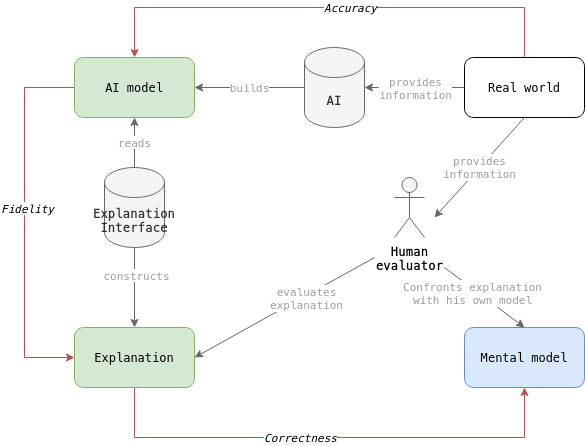
\includegraphics[width=\linewidth]{images/evaluation.png} \caption{Evaluation process of an AI through an explanation interfaces.} \label{fig:eval} \end{figure}

A problem that can be present in this situation is the fact that the AI model and the representation chosen for the explanation could be of very different nature, such as in Causal Models described in Section~\ref{sec:solutions}. If that is the case, does it even make sense to ask ourselves if a causal relationship ``really'' represents the AI model, which typically learns using statistical correlation? And if, on the other hand, both the AI and the explanation are black boxes, how can we be sure that evaluating the AI using that explanation interface will effectively improve our understanding of the underlying AI model? Could we just \textit{think} we are understanding it?

\subsection{Decision making biases}
\label{sec:bias}

Human decision-making is known to be affected by many cognitive bias, which are deeply rooted in our thinking and are often difficult, if not impossible, to exclude when we make decisions. Recently, \citet{framingeffect} has studied the consequences of the \textit{framing effect} in the domain of AI, in particular how likely is a person to accept or reject an AI recommendation based on how the output was framed. An interesting result of this research is, for example, that ``\textit{perceived reasonableness was significantly higher when the suggestion of AI was provided before the decision is made than after the decision is made when perceived accuracy was controlled}''.

While this is not a direct study on AI explanation interfaces, it does show how the same local decision of an AI can be judged differently just varying the timing of the explanation, and a similar result is found about the way the solution is framed.

This goes to show how the evaluation of the correctness of an AI model is not only a subjective matter, but can vary in the same individual depending on factors that are external to the AI behavior itself.

\subsection{Can explanation interfaces learn to exploit cognitive bias?}
\label{sec:exploit}

As a pure thought experiment, let's imagine a situation where a single individual is in charge of deciding whether an explanation interface is suited for understanding a certain type of AI architecture, e.g. Neural Networks, and let's make the assumption that the only observable elements are the output of the AI model and the explanation provided by the interface. This settings is not far from the one of an operator who acts upon AI recommendations. Let's then suppose that the explanation interface is a complex interface that can convert the model's internals into a human-like reasoning, for example by producing textual motivations for a certain output.

As we demonstrated, it is completely possible that the judgment about the correctness of the algorithm is biased by the way the explanation interface presents the information. Let's now suppose that the same individual has to choose between multiple explanation interfaces and multiple AI models the best couple of model-explainer to be put in production: even if the single explanation interface is not built to learn from the individual's taste, this environment creates a selection for those explanation systems that present information in a way that fits better the idea the individual has about the problem. In particular, an feasible solution to this problem could be a couple in which the explainer is very convincing at justifying the AI model. In absence of other information, the individual has equal probability of selecting the most correct explanation interface and the most accurate AI model, or the most convincing explanation interface coupled with a sub-optimal model.

In this way, we have created a scenario in which an explanation interface that can lie very well is indistinguishable from a very accurate explanation of a convincing model.

%-----------------------------------------------------------------%
\section{Conclusions}
\label{sec:conclusions}

% critiques:
% 1. allora non si può fare niente per migliorare l'interpretabilità?
% 2. le AI mica hanno lo scopo di fotterti
% 3. c'è lo stesso problema con ogni rappresentazione allora
% 4. si può fixare se valuti quanto la spiegazione incrementa la predittività
%           sì ma c'è sempre il problema del test set vs vita reale

In conclusion, we have showed how the fact that there is no single definition of what interpretability is and no comprehensive way of evaluating all important aspects that compose an explanation leads to the possibility of creating yet another black-box layer over the black-box model, which can accentuate biases instead of reducing them.

Some criticisms that can be made to this argument are:

\begin{itemize}
    \item Does it mean that all XAI solutions are useless? Absolutely not. This is an important research that is fundamental for the future of AI, and the fact that many directions are being explored to solve this problem is just a reflection of how multi-faceted is the problem itself.
    \item Can't the problem stated in \ref{sec:exploit} be overcome by simply adding more judges? While this is true, the problem of cognitive bias is that it can also be inherited from the group or society around the single individual. Certainly, a diverse control group for evaluating explanations is a must-have, but it is not a complete guarantee of absence of bias.
    \item Can't errors introduced by the explanation interface be simply corrected by looking at the actual behavior of the AI? If the explanation itself behaves more or less like a black-box, i.e. in those cases in which it is difficult to quantify the explanation's fidelity, there is the same problem that affects AI testing in general: even if testing is done extensively and all results are positive, i.e. the explanation is always perfectly aligned to the AI model, we have no general guarantee that this holds for all the possible outcomes.
\end{itemize}

In the end, while the proposed argument is just a thought experiment, there are many elements which are realistic and should be paid attention to when devising XAI solutions.

\bibliographystyle{plainnat}
\bibliography{references}

\end{document}
